\subsection{Networked Simulator}
\label{sec:netsim}
The networked simulator consists of the proxy server (\texttt{ProxyServerNet}) and the mobile client 
simulator (\texttt{SimulatorV3} run on a departmental Ubuntu server), which is a wrapper for the 
networked mobile proxy-client (\texttt{MobileClientNet}) and is capable of performing several rounds 
of requests to the proxy server in real-time. It does so by prompting the user to manually enter the 
next web page URL she wishes to visit, simulating web browser interactions. The simulator architecture 
can be seen in Figure \ref{fig:netsim_arch}. 

\begin{figure}[ht]
\centering 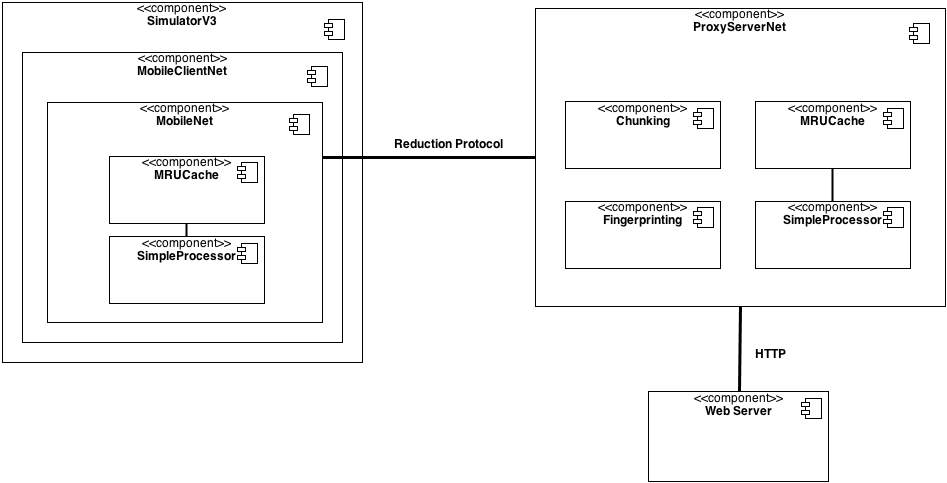
\includegraphics[width=\columnwidth]{images/component_diagram.png}
\caption{Networked Simulator Runtime Interactions.}
\label{fig:netsim_arch}
\end{figure}

In more detail, the networked simulator implements our reduction protocol as follows. First, the 
mobile proxy-client opens a socket to the proxy server, which is listening for connections at a user-
specified port. The mobile proxy-client sends an HTTP request to the proxy server, which in turn sends it on to the hosting web server, including the User-Agent string of a mobile device\footnote{We use the Samsung Galaxy SII as our model mobile device across all our implementations and experiments.} to ensure that it receives the mobile version of the requested web page. Once the proxy has received the response from the appropriate web server, it engages in our protocol\footnote{Minor changes were made to the chunking facility as well as the mobile device definition to support networking.} with the mobile proxy-client, exchanging the relevant information via the network. At the end, the mobile proxy-client reconstructs the content data of the received web page into an HTML file, which can then be viewed in any web browser. After the proxy has served the mobile client's request, the client is able to make a new request and repeat this process.

We found that, while simulating mobile browsing, for one not using an actual mobile phone, and for 
another not using a web browser program of any sort, is not realistic, our networked simulator is a 
good first proof-of-concept prototype showing that our reduction protocol is viable. In our 
experimental evaluation, we argue that it reduces the required bandwidth compared to the currently 
required mobile browsing bandwidth.

In the end, we would like to discuss some caveats of our networked simulator. First, as our mobile 
client simulator does not have the capabilities of a web browser and it receives preprocessed data 
from the proxy server, it cannot automatically handle HTTP responses indicating page redirects (i.e. 
server response code $301$, for example). Thus, our proxy server handles HTTP responses with the 
server response codes $200$ and $40X$\footnote{$200$ means granted normally, $40X$ response codes 
indicate a form of client-side error such as malformed requests but return HTML-format content with 
this information.} since the web server returns HTML content with these responses. An additional 
consequence of the fact that our mobile client is not browser-like is that it must create a local copy 
of each retrieved web page. Although the content of the web page is reconstructed correctly, since 
many links within web pages point to relative paths, the retrieved web pages are often rendered 
incorrectly in the local web browser as it cannot find cascading stylesheets (CSS) and embedded images 
on the local disk. We propose how to solve these issues in our discussion on future work.